\section{Released Artifacts and Reproducibility}
\label{app:artifacts}

\subsection{Released artifacts}

\begin{itemize}\itemsep -1pt
  \item \textbf{Dataset (HuggingFace).}
    \url{https://huggingface.co/datasets/oenobench/oenobench} —
    \texttt{release\_v1.2}, 3{,}266 questions, Parquet test split,
    \texttt{README.md} datasheet, \texttt{croissant.json} manifest.
    License: CC-BY-SA-4.0. Versioning is permanent: prior releases
    remain accessible via revision tags.
  \item \textbf{Code (GitHub).}
    \url{https://github.com/nikitahudov/oenobench} — full pipeline:
    35 scrapers, 5 question generators, 9 audit agents, the human
    review web app, and the monitoring dashboard. Apache 2.0.
  \item \textbf{Pipeline diagrams.} Included in
    \texttt{docs/figures/} as Mermaid (.mmd), PNG, and SVG.
  \item \textbf{Process log.} \texttt{docs/PROCESS\_LOG.md} —
    chronological lab-notebook of every phase shipped, with sources,
    methodology, quality-control counts, and decision rationale, in
    the format prescribed for the methodology sections of this paper.
  \item \textbf{Audit reports.} \texttt{docs/QUALITY\_AUDIT\_REPORT.md},
    \texttt{docs/RELEASE\_V1\_2\_AUDIT\_ACTIONS.md},
    \texttt{docs/GOLD\_CALIBRATION\_ANALYSIS.md},
    \texttt{data/reports/zero\_correct\_97\_audit.md}.
  \item \textbf{Eval reports.}
    \texttt{data/reports/eval\_release\_v1\_2\_full\_cleaned.md} (the
    16-config × 3{,}266-Q run reported in this paper).
\end{itemize}

\subsection{Reproducibility scripts}

The construction pipeline is driven by a small number of shell scripts
in \texttt{scripts/}:

\begin{itemize}\itemsep -1pt
  \item \texttt{run\_all\_scrapers.sh} — orchestrates the 35 scrapers
    end-to-end. Each scraper writes a timestamped log to
    \texttt{data/logs/}.
  \item \texttt{run\_release\_v1\_build.sh} — full generation pipeline
    invocation; idempotent and resume-safe via stamped tags.
  \item \texttt{export\_release\_v1\_2\_to\_parquet.py} — produces the
    HuggingFace Parquet directly from Postgres; the released file
    is the byte-identical output of this script.
  \item \texttt{build\_smart\_review\_sheet.py} — generates a 50-question
    stratified gold-sheet review batch (random + critical-FAIL +
    borderline-WARN strata).
  \item \texttt{tag\_audit\_actions.py} — applies the audit drop /
    relabel policy to a tagged corpus; this is the script that
    produced the \texttt{release\_v1.2} state from
    \texttt{release\_v1.1}.
\end{itemize}

\subsection{Database schema}

The released schema is initialised by the migrations under
\texttt{config/postgres/} (six idempotent files, applied in order on
container startup):
\texttt{init.sql} (sources, facts, questions, question\_facts,
generation\_metadata, evaluation\_runs, evaluation\_answers,
human\_reviews),
\texttt{002\_audit\_schema.sql} (audit\_runs, audit\_findings,
audit\_gold\_labels, audit\_severity enum),
\texttt{003\_sample\_schema.sql} (mirror schema for the Phase~5
sample-DB eval),
\texttt{003\_cb\_reserve.sql} (closed-book reserve pool tagging),
\texttt{004\_eval\_telemetry.sql} (provider, tokens, reasoning\_config,
latency columns on \texttt{evaluation\_answers}),
\texttt{005\_or\_cost\_telemetry.sql} (OpenRouter authoritative cost
columns).

A simplified entity-relationship diagram is in
Figure~\ref{fig:schema}.

\begin{figure}[h]
  \centering
  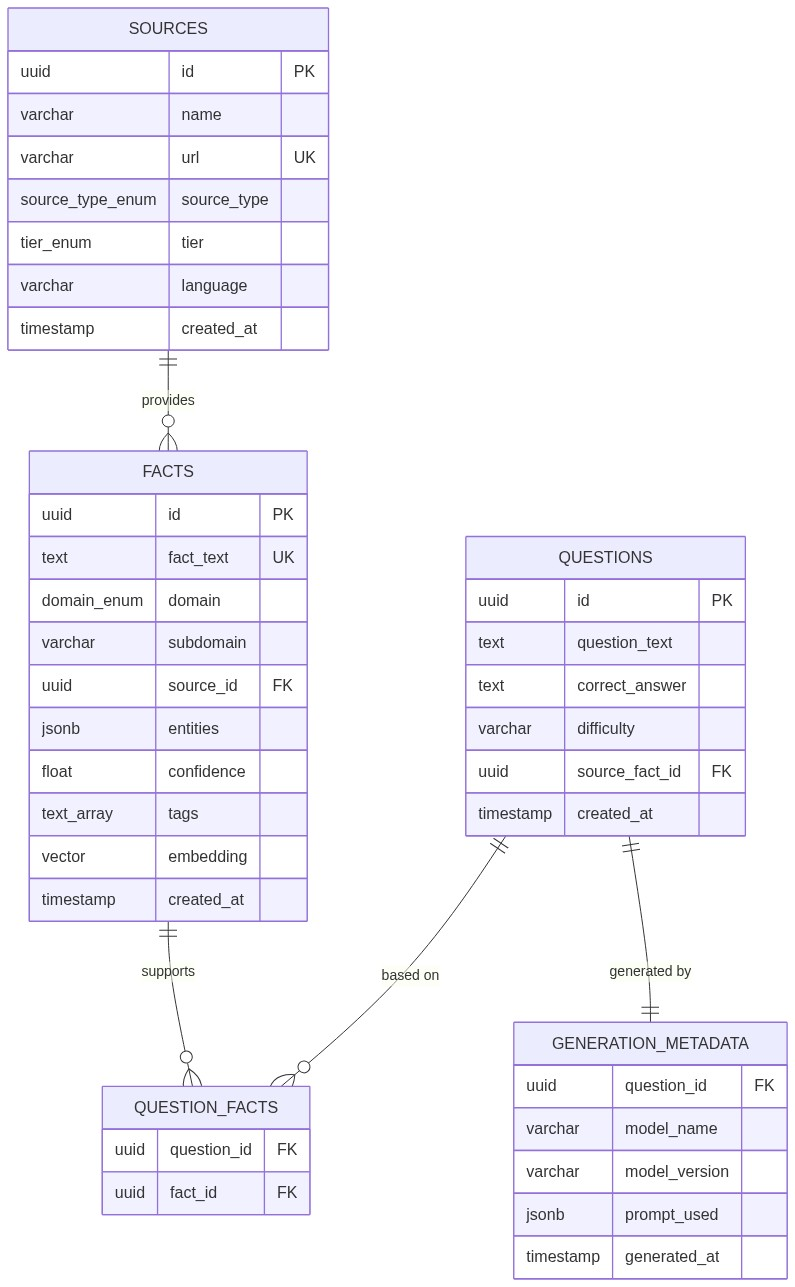
\includegraphics[width=0.85\linewidth]{figures/diagram_schema.png}
  \caption{Simplified release schema. \texttt{sources} ground
    \texttt{facts}; \texttt{questions} pull from \texttt{facts} via
    \texttt{question\_facts}; \texttt{generation\_metadata} records
    the LLM and strategy that produced each question;
    \texttt{audit\_findings} holds per-agent verdicts;
    \texttt{human\_reviews} holds gold-sheet ratings.}
  \label{fig:schema}
\end{figure}

\subsection{Compute and cost}

The full evaluation reported in Section~\ref{sec:eval} ran in
\textbf{120 minutes 34 seconds} on a single VM driving 16 OpenRouter
configurations in parallel. Total LLM API spend across construction
was approximately:
\begin{itemize}\itemsep -1pt
  \item Generation pipeline: \$160 (across audit pilots v1--v16 and
    the final \texttt{release\_v1} build).
  \item Audit pipeline (release\_v1.2 cycle): \$76.
  \item Evaluation (16 configs × 3{,}266 Q): \$98.33 effective
    OpenRouter cost.
\end{itemize}
No GPU compute was used; all model inference was via OpenRouter (a
unified API gateway). The release artefacts include all per-call
telemetry (provider, tokens, reasoning configuration, p50/p95
latency, OR-authoritative cost) for the full evaluation run.

\subsection{Test status}

771 of 771 unit tests pass on \texttt{main} as of the camera-ready
build. Tests cover the fact-processing pipeline, the five generation
strategies, all nine audit agents, the orchestrator, the closed-book
gate, the eval harness (slot dispatch, cost computation,
reasoning-mode prompt assembly), and the review-app endpoints.

\subsection{Anonymisation note}

For double-blind submission, the public-facing URLs in this paper are
mirrored to anonymous fora as documented in \texttt{docs/ANONYMIZATION\_PLAN.md}.
The HuggingFace dataset is mirrored at an anonymous handle, the
GitHub repository is exposed via \texttt{anonymous.4open.science}, and
all author/funding declarations are blanked in the OpenReview
submission. The camera-ready will swap all anonymous URLs back to
their canonical equivalents; the mapping is preserved in the
anonymisation plan file in the released code.
